%%%%%%%%%%%%%%%%%%%%%%%%%%%%%%%%%%%%%%%%%
% Short Sectioned Assignment
% LaTeX Template
% Version 1.0 (5/5/12)
%
% This template has been downloaded from:
% http://www.LaTeXTemplates.com
%
% Original author:
% Frits Wenneker (http://www.howtotex.com)
%
% License:
% CC BY-NC-SA 3.0 (http://creativecommons.org/licenses/by-nc-sa/3.0/)
%
%%%%%%%%%%%%%%%%%%%%%%%%%%%%%%%%%%%%%%%%%

%----------------------------------------------------------------------------------------
%	PACKAGES AND OTHER DOCUMENT CONFIGURATIONS
%----------------------------------------------------------------------------------------

\documentclass[paper=a4, fontsize=11pt]{scrartcl} % A4 paper and 11pt font size

\usepackage[T1]{fontenc} % Use 8-bit encoding that has 256 glyphs
\usepackage{fourier} % Use the Adobe Utopia font for the document - comment this line to return to the LaTeX default
\usepackage[english]{babel} % English language/hyphenation
\usepackage{amsmath,amsfonts,amsthm} % Math packages

\usepackage{lipsum} % Used for inserting dummy 'Lorem ipsum' text into the template
\usepackage{graphicx}

\usepackage{sectsty} % Allows customizing section commands
\allsectionsfont{\centering \normalfont\scshape} % Make all sections centered, the default font and small caps

\usepackage{fancyhdr} % Custom headers and footers
\pagestyle{fancyplain} % Makes all pages in the document conform to the custom headers and footers
\fancyhead{} % No page header - if you want one, create it in the same way as the footers below
\fancyfoot[L]{} % Empty left footer
\fancyfoot[C]{} % Empty center footer
\fancyfoot[R]{\thepage} % Page numbering for right footer
\renewcommand{\headrulewidth}{0pt} % Remove header underlines
\renewcommand{\footrulewidth}{0pt} % Remove footer underlines
\setlength{\headheight}{13.6pt} % Customize the height of the header

\numberwithin{equation}{section} % Number equations within sections (i.e. 1.1, 1.2, 2.1, 2.2 instead of 1, 2, 3, 4)
\numberwithin{figure}{section} % Number figures within sections (i.e. 1.1, 1.2, 2.1, 2.2 instead of 1, 2, 3, 4)
\numberwithin{table}{section} % Number tables within sections (i.e. 1.1, 1.2, 2.1, 2.2 instead of 1, 2, 3, 4)

\setlength\parindent{0pt} % Removes all indentation from paragraphs - comment this line for an assignment with lots of text

%----------------------------------------------------------------------------------------
%	TITLE SECTION
%----------------------------------------------------------------------------------------

\newcommand{\horrule}[1]{\rule{\linewidth}{#1}} % Create horizontal rule command with 1 argument of height

\title{	
\normalfont \normalsize 
\textsc{University of Iowa, Professor Omar Haider} \\ [25pt] % Your university, school and/or department name(s)
\horrule{0.5pt} \\[0.4cm] % Thin top horizontal rule
\huge Databases in OpenEMR \\ % The assignment title
\horrule{2pt} \\[0.5cm] % Thick bottom horizontal rule
}

\author{Junhyuk Kang} % Your name

\date{Sep 20, 2016 ~ Sep 26, 2016 } % Today's date or a custom date


\begin{document}

\maketitle % Print the title

%----------------------------------------------------------------------------------------
%	PROBLEM 1
%----------------------------------------------------------------------------------------
\section{Assignments}
\begin{enumerate}
  \item Show all Tables / Columns
  \item Show ACL (Access Control List)
  \item Where is detail log stored (Who logged in? Patients' log)
\end{enumerate}
%----------------------------------------------------------------------------------------
%	PROBLEM 2
%----------------------------------------------------------------------------------------

\section{Answer Steps}

%------------------------------------------------
\begin{itemize}
	\item Tried to show all columns in database with 'show' command but did not work
		\begin{itemize}
		\item
		 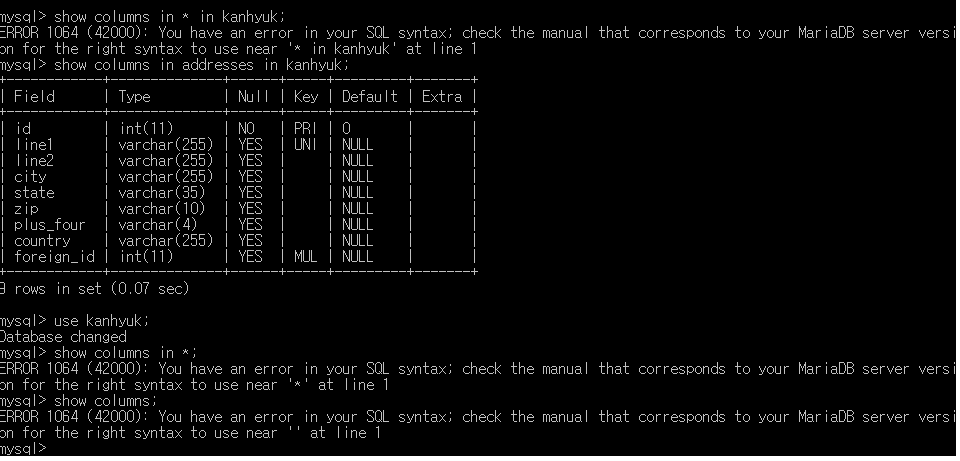
\includegraphics[width = 20cm, height=7cm]{pictures/selectcoler.jpg}
		\end{itemize}
	\item Use database by using 'use 'database name''
	\item Changed command to 'select * from 'database name''
		\begin{itemize}	
			\item Result of 'select * from users' (Users contains  user data)
			\item
			 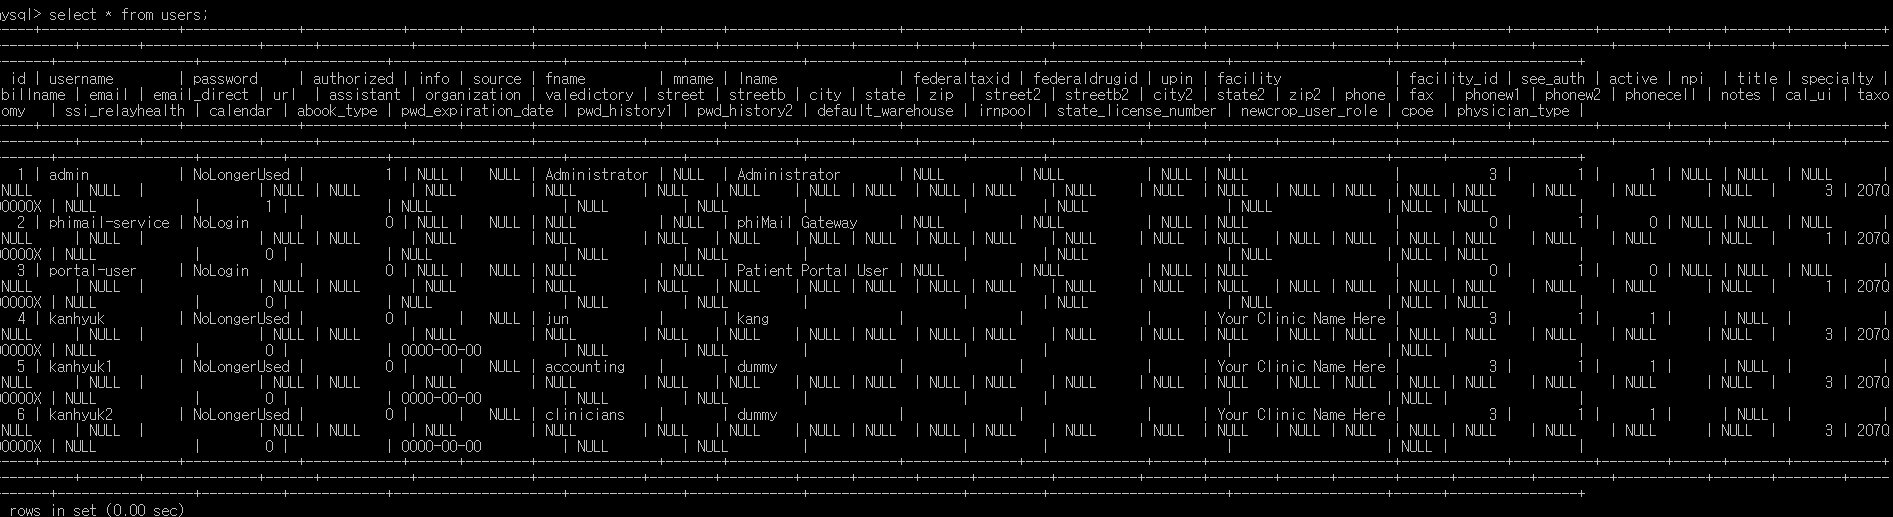
\includegraphics[width = 35cm, height=8cm]{pictures/userdata.png}
		\end{itemize}
	\item We can check data in each column by 'select'
	\item Tried to find every data in my database by using select
	\item Found detail user log in 'log' column
		\begin{itemize}	
			\item
			 \includegraphics[width = 35cm, height=10cm]{pictures/LOGDATADETAIL.png}
			\item In detail, it shows who accessed to openemr and what did they do
			\item 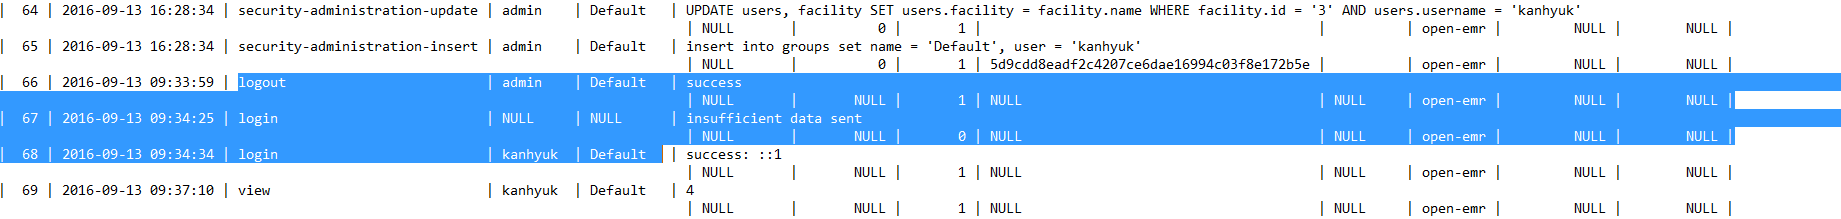
\includegraphics[width = 35cm, height=5cm]{pictures/whologinlog.png}
\vspace{5cm}
			\item After I found column, I tried to find log file
			\item 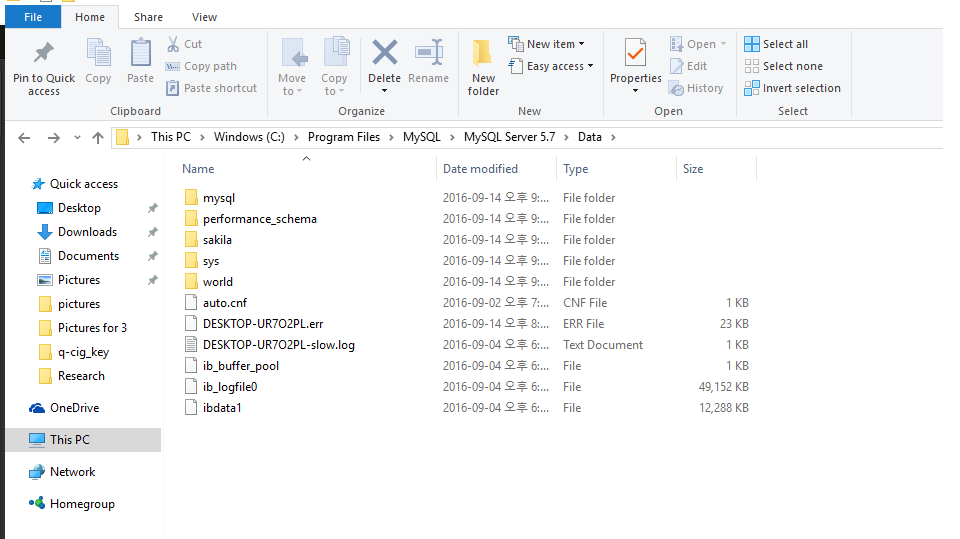
\includegraphics[width = 10cm, height=5cm]{pictures/wherelog.png}
			\item all data are in 'DATA' folder, and log file is in $ib_logfile$
			
		\end{itemize}
	\item Found message log on 'pnotes' column
		\begin{itemize}	
			\item
			 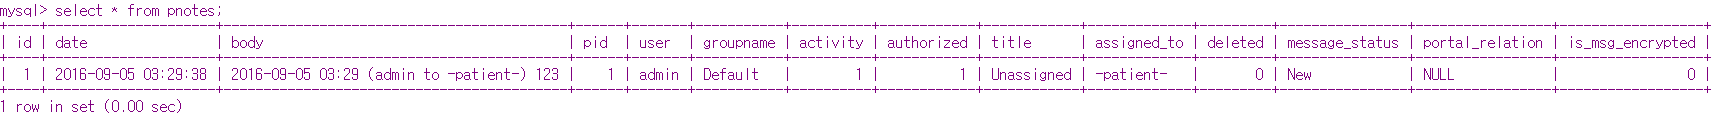
\includegraphics[width = 35cm, height=5cm]{pictures/wherepnotes.png}
		\end{itemize}
	\item Found where is username, password data stored in $'users_secure'$ column
		\begin{itemize}	
			\item
			 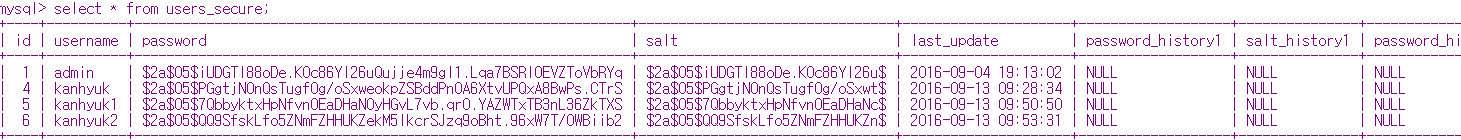
\includegraphics[width = 35cm, height=5cm]{pictures/wherepassword.png}
		\end{itemize} 
\vspace{3cm}
	\item Found access control list on $'gacl_acl'$ column
		\begin{itemize}	
			\item Shows different access depends on their login status(ex. Admin or Clinicians)
			\item
			 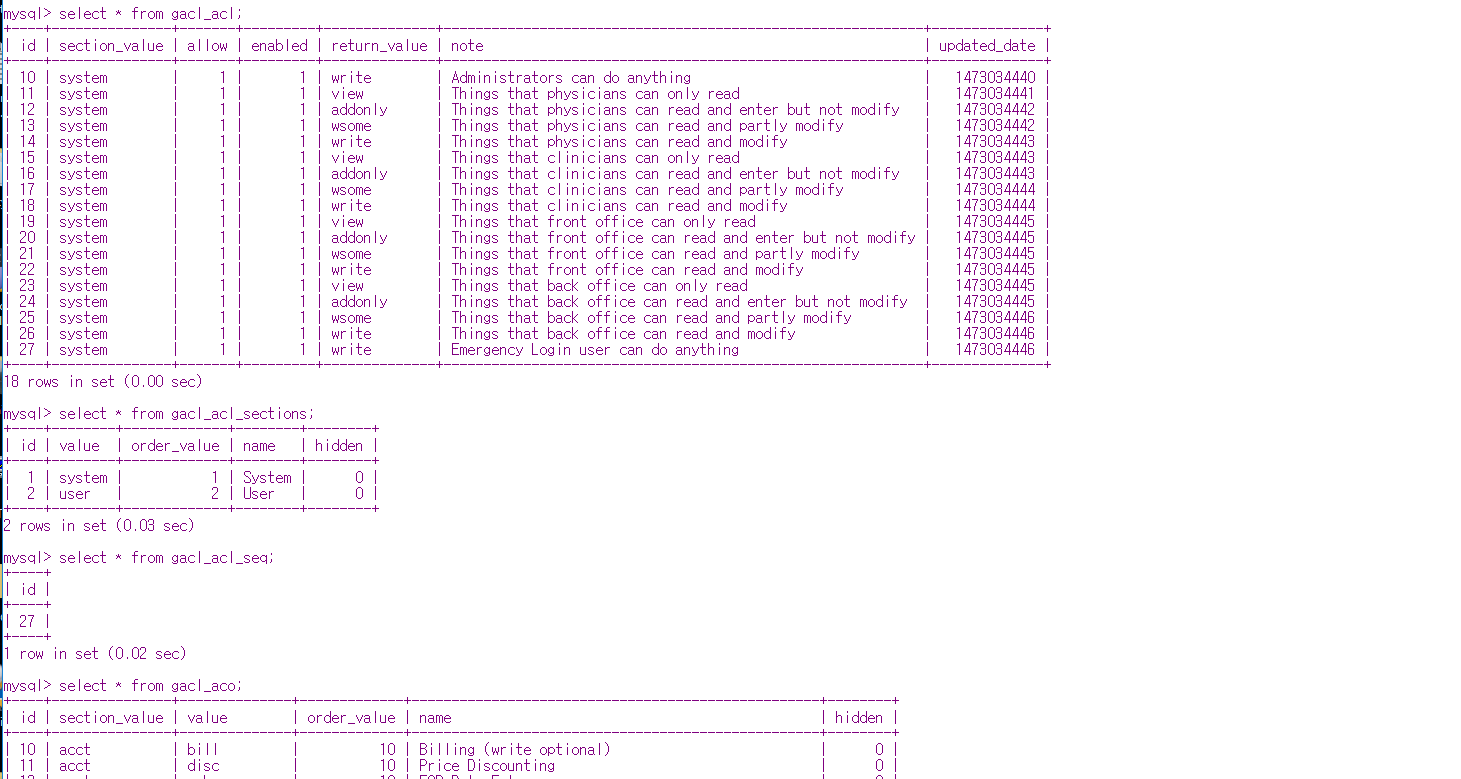
\includegraphics[width = 35cm, height=15cm]{pictures/authorities.png}
		\end{itemize}
	\item Most of the other columns were empty but found
		\begin{itemize}	
			\item Popup Message log(ex. stop smoking) in $'clinical_reules_log'$ column
			\item Diseases codes in 'codes' column
			\item History of data in $'history_data' column'$
			\item Automatic welcome messages in $'automatic_notification'$ column
		\end{itemize}
\vspace{3cm}
	\item Tried to work on MySQL work bench
		\begin{itemize}	
			\item Found my databases under 'schemas'
			\item Tried to open it with double click but just copied database name on query
			\item Applied same command on query (use, and select to access to my database)
			\item 	
			 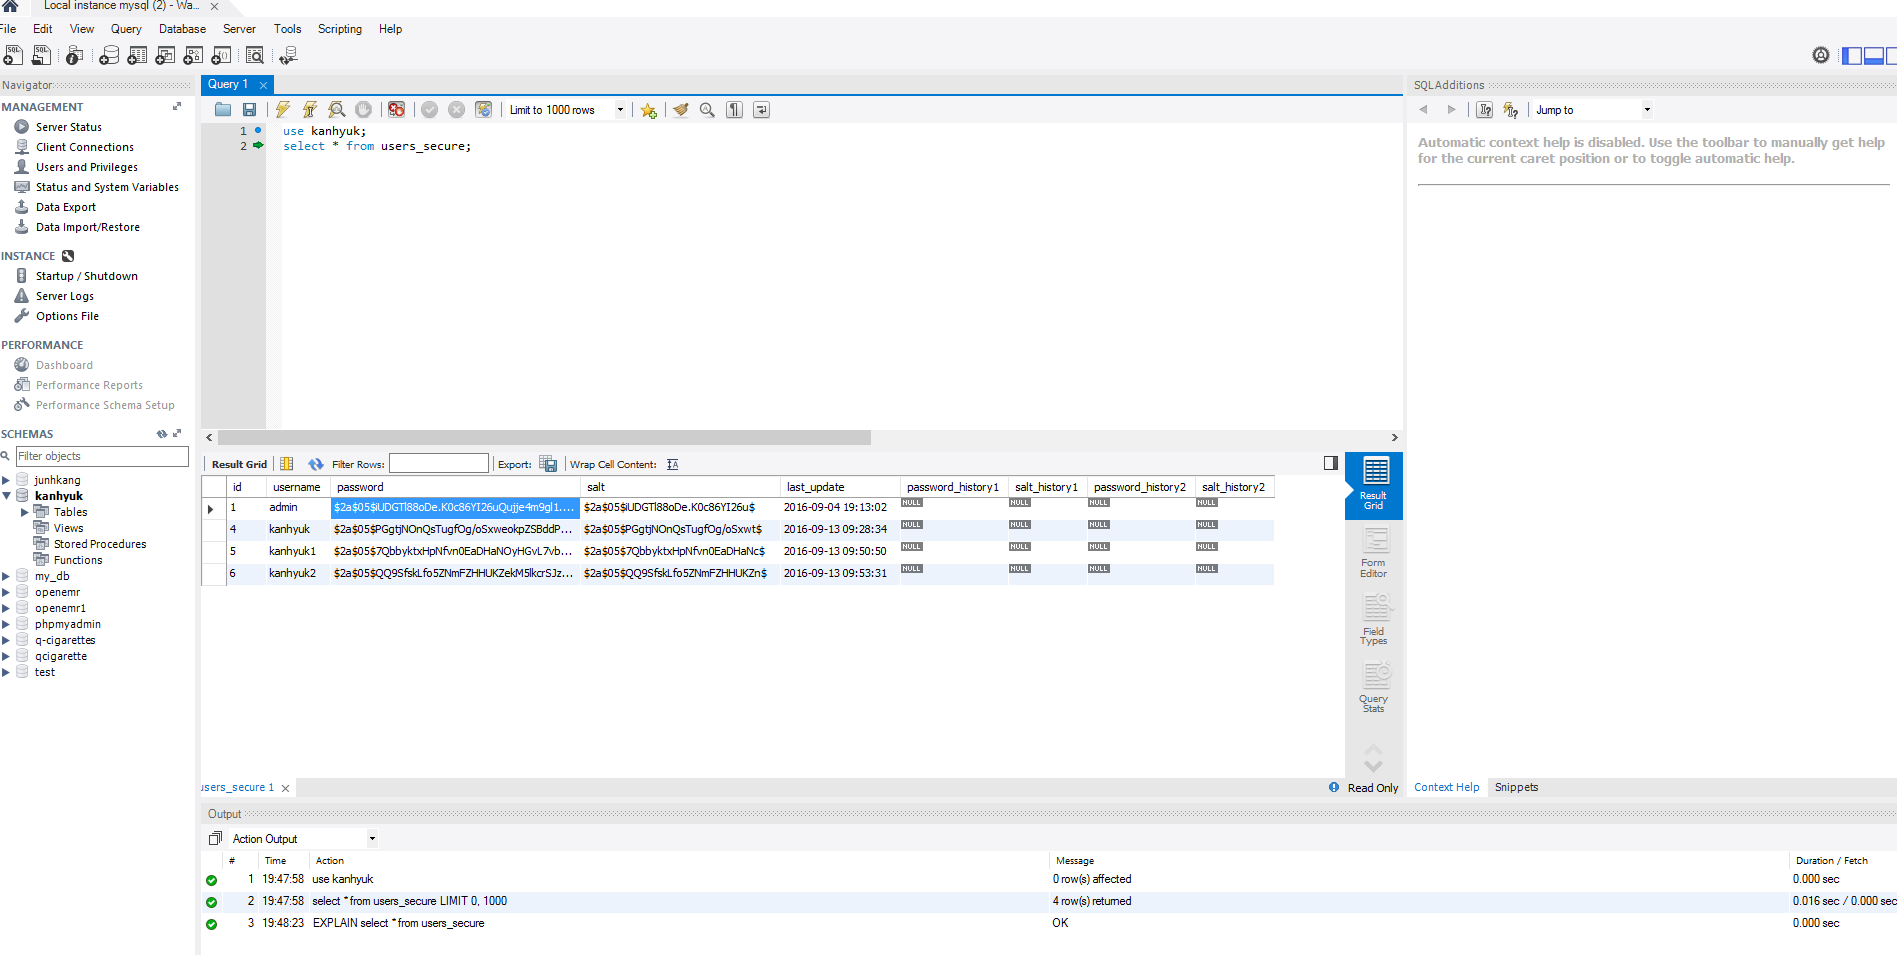
\includegraphics[width = 25cm, height=10cm]{pictures/worbetchdatabase.png}
		\end{itemize}


	\end{itemize}







\end{document}